\documentclass[12pt]{article}
\usepackage[utf8]{inputenc}
\usepackage{amsmath,amssymb}
\usepackage{float}
\usepackage{graphicx}
\usepackage[a4paper, margin=2cm]{geometry}
\usepackage{enumerate}
\usepackage{xcolor}
\usepackage{caption}
\usepackage{tikz}
\usepackage{tikz-3dplot} % Permite coordenadas 3D
% Definir un comando para el número de pregunta en azul
\newcommand{\question}[1]{\textcolor{blue}{\textbf{#1}}}
%\usepackage[spanish]{babel}
\begin{document}
\begin{titlepage}
        \begin{center}
            \LARGE \textbf{Taller No. 3\\Teoría Electromagnética}
            \vfill
            \large

            Karen Alejandra Freire Rosero\\
            Sonier Andrés Ortiz Castelblanco\\
            Sarah Isabel Tejada García\\
            Santiago Alejandro Pérez Ramos
            \vfill
            \textbf{Asignatura:} Teoría Electromagnética\\
            \textbf{Profesor:} Servio Tulio Pérez Merchancano, Ph.D\\
            \vfill
            Universidad del Cauca\\
            Facultad de Ciencias Naturales, Exactas y de la Educación\\
            Departamento de Física\\
            Popayán, Cauca\\
            2025
        \end{center}
\end{titlepage}
%---------------------------------------------Ej_20_IDMCh---------------------------------
\section*{\question{ Problema 2.20}} Uno de estos es un campo electrostático imposible. ¿Cuál?

\begin{enumerate}[(a)]
    \item  \(\mathbf{E} = k[xy \mathbf{ \hat{x}}+ 2yz\mathbf{ \hat{y}}+ 3zx\mathbf{ \hat{z}}] \)
    \item \(\mathbf{E} = k[y^2\mathbf{ \hat{x}}+ (2xy + z^2)\mathbf{ \hat{y}}+ 2zx\mathbf{ \hat{z}}] \)
\end{enumerate}

Donde \(k\)  es una constante con las unidades adecuadas. Para el campo posible, encuentre el potencial \(V\), usando el origen como punto de referencia. Verifique su respuesta calculando el \(\nabla V\) y comparando con el campo eléctrico que encontró en el inciso a.(Pista: Debe elegir una trayectoria específica para integrar. La respuesta es independiente de la trayectoria, pero no puede integrar sin definir una.)

\subsection*{Solución:}
Para un campo electrostático, el rotacional del campo eléctrico debe ser cero. Por lo tanto, para determinar si un campo es electrostático o no, debemos calcular el rotacional de cada uno de los campos eléctricos propuestos.

\subsubsection*{Para el campo (a)}

Calculo del rotacional el rotacional:

\[
\nabla \times \mathbf{E} = 
\begin{vmatrix}
\hat{\mathbf{x}} & \hat{\mathbf{y}} & \hat{\mathbf{z}} \\
\partial_x & \partial_y & \partial_z \\
kxy & 2k yz & 3k xz
\end{vmatrix}
\]

\begin{align*}
(\nabla \times \mathbf{E})_x &= \frac{d}{dy} (3kxz) - \frac{d}{dz} (2kyz) = 0 - 2ky = -2ky \\
(\nabla \times \mathbf{E})_y &= \frac{d}{dz} (kxy) - \frac{d}{dx} (3kxz) = 0 - 3kz = -3kz \\
(\nabla \times \mathbf{E})_z &= \frac{d}{dx} (2kyz) - \frac{d}{dy} (kxy) = 0 - kx = -kx
\end{align*}

\[
\nabla \times \mathbf{E} = -2ky\,\hat{\mathbf{x}} - 3kz\,\hat{\mathbf{y}} - kx\,\hat{\mathbf{z}} \neq \mathbf{0}
\]


\boxed{\text{El campo (a) es imposible}}


\subsubsection*{Para el campo (b)}
Calculamos el rotacional:

\[
\nabla \times \mathbf{E} = 
\begin{vmatrix}
\hat{\mathbf{x}} & \hat{\mathbf{y}} & \hat{\mathbf{z}} \\
\partial_x & \partial_y & \partial_z \\
ky^2 & k(2xy + z^2) & 2kyz
\end{vmatrix}
\]

\begin{align*}
(\nabla \times \mathbf{E})_x &= \frac{d}{dy} (2kyz) - \frac{d}{dz} (kz^2) = 2kz - 2kz = 0 \\
(\nabla \times \mathbf{E})_y &= \frac{d}{dz} (ky^2) - \frac{d}{dx} (2kyz) = 0 - 0 = 0 \\
(\nabla \times \mathbf{E})_z &= \frac{d}{dx} (2kxy) - \frac{d}{dy} (ky^2) = 2ky - 2ky = 0
\end{align*}

\[
\nabla \times \mathbf{E} = \mathbf{0}
\]

\subsection*{Cálculo del potencial para (b)}
Integrando a lo largo de la trayectoria \((0,0,0) \to (x,0,0) \to (x,y,0) \to (x,y,z)\):

\begin{figure}[h]
    \centering
    \tdplotsetmaincoords{70}{120} % ángulo de vista

    \begin{tikzpicture}[tdplot_main_coords, scale=3]

        % Ejes coordenados
        \draw[->] (0,0,0) -- (1.5,0,0) node[anchor=north east]{$x$};
        \draw[->] (0,0,0) -- (0,1.5,0) node[anchor=north west]{$y$};
        \draw[->] (0,0,0) -- (0,0,1)   node[anchor=south]{$z$};

        % Coordenadas de trayectoria
        \coordinate (a) at (1,0,0);
        \coordinate (b) at (1,1,0);
        \coordinate (c) at (1,1,1); % Este es el punto final

        % Trayectoria en pasos
        \draw[thick, red, ->] (0,0,0) -- (a) node[anchor=south east] {$(x_0)$} node[midway , above] {$\lambda_1$};
        \draw[thick, blue, ->] (a) -- (b) node[anchor=south west] {$(y_0)$} node[midway , above] {$\lambda_2$};
        \draw[thick, green, ->] (b) -- (c) node[anchor=north west] {$(z_0)$} node   [midway , right] {$\lambda_3$};

        % Punto final
        \filldraw[black] (c) circle (0.5pt);
        \node[anchor=south] at (c) {$(x_0, y_0, z_0)$};

    \end{tikzpicture}
    \caption*{Trayectoria $(x_0, y_0, z_0)$}
\end{figure}




Parametrizando  la trayectoria con respecto a un parametro \(t\) 
\[ \lambda = \lambda_1 + \lambda_2 + \lambda_3\]
\[
\lambda[0, r_0]: \longrightarrow  \mathbf{R^3}   
\]
% preguntar al profe por la notación de la trayectoria
\[ \lambda_1 = (t,0,0),\, \lambda_1' = (1,0,0)dt \]
\[ \lambda_2 = (0,t,0),\, \lambda_2' = (0,1,0)dt \]
\[ \lambda_3 = (0,0,t),\, \lambda_3' = (0,0,1)dt \]
\[
V(x,y,z) = -\int_0^{x_0} \mathbf{E}\cdot d \lambda_1' -\int_0^{y_o} \mathbf{E}\cdot d \lambda_2'-\int_0^{z_0} \mathbf{E}\cdot d \lambda_3'
\]

\begin{align*}
    \int_0^{x_0} \mathbf{E}\cdot d \lambda_1'& =  \int_0^x k((0)^2,[2(t)(0) + 0^2],2(0)) \cdot (1,0,0)dt\\
& = 0
\end{align*}

\begin{align*}
    \int_0^{y_0} \mathbf{E}\cdot d \lambda_2'& =  \int_0^{y_0} k((t)^2,[2(x_o)(t) + 0^2],2(0)(t)) \cdot (0,1,0)dt\\
& = \int_0^{y_0} k((t)^2,[2(x_0)(1) + 0^2],2(0)(t)) \cdot (0,1,0)dt\\
& = \int_0^{y_0} 2kx_o t dt\\
& = kx_0 t^2 \bigg|_0^{y_0} \\
& = kx_0 y_0^2
\end{align*}

\begin{align*}
    \int_0^{z_0} \mathbf{E}\cdot d \lambda_2'& =  \int_0^{z_0} k((yo)^2,[2(x_o)(y_0) + t^2],2(t)(y_0)) \cdot (0,0,1)dt\\
    & = \int_0^{z_0} k((y_0)^2,[2(x_0)(y_0) + t^2],2(t)(y_0)) \cdot (0,0,1)dt\\
    & = \int_0^{z_0} 2ky_o t dt\\
    & = ky_0 t^2 \bigg|_0^{z_0} \\
    & = ky_0 z_0^2
\end{align*}

\begin{align*}
    V(x,y,z)& = -kx_0 y_0^2 - ky_0 z_0^2\\
& =-k[x_0y_0^2 + y_0z_0^2] \\
\end{align*}
En general 
\[\boxed{ V(x,y,z) = -k(xy^2 + yz^2)}\]


Verificación, calculando el Gradiente del potencial:
\begin{align*}
    \nabla V & = \left(\frac{\partial V}{\partial x}, \frac{\partial V}{\partial y}, \frac{\partial V}{\partial z}\right) \\
    \nabla V & = \left(-k(y^2), -k(2xy + z^2), -k(2yz)\right) \\
    \nabla V  & = -k\left(y^2\,\hat{\mathbf{x}} + (2xy + z^2)\,\hat{\mathbf{y}} + 2yz\,\hat{\mathbf{z}}\right) = -\mathbf{E}
\end{align*}

\[
    \boxed{V(x,y,z) = -k(xy^2 + yz^2)}
\]


%--------------------------------------------Ej_22_IDMCh---------------------------------
\section*{\question{ Problema 2.22}} Hallar el potencial eléctrico V a una distancia s de un alambre recto infinitamente largo que transporta una carga lineal uniforme \(\lambda\)

\subsection*{Solución:}
Para encontrar el potencial \(V\) de un campo eléctrico dado,  usamos la integral de línea del campo eléctrico sobre una trayectoria que va desde el punto \((0,0,0)\) hasta el punto \((x,y,z)\)
\[
\mathbf{V(s)} = -\int_{0}^{\mathbf{r}} \mathbf{E}\cdot d \mathbf{l}   
\]    

para un alambre recto infinitamente largo, el campo eléctrico es radial y tiene la forma:
\[
\mathbf{E} = \frac{\lambda}{2\pi \epsilon_0 s} \hat{\mathbf{s}}
\]

Reemplazando en la integral de línea, tenemos:
\[
    \mathbf{V(s)} = -\int_{0}^{s} \frac{\lambda}{2\pi \epsilon_0 s} ds 
\]
\[
\boxed{\mathbf{V(s)} =  -\frac{\lambda}{2\pi \epsilon_0} \ln(s) }
\]

Para comprobar el resultado, calculamos el campo eléctrico a partir del potencial:
Además, dado que el sistema esta en coordenadas cilíndricas el campo eléctrico se puede calcular como:

\begin{align*}
    \mathbf{E}  &= -\nabla V = -\frac{\partial V}{\partial s} \hat{s} \\
    \mathbf{E} &= -\frac{\partial}{\partial s} \left(-\frac{\lambda}{2\pi \epsilon_0} \ln(s) \right) \\
    \mathbf{E} &= \frac{\lambda}{2\pi \epsilon_0} \frac{1}{s} \hat{\mathbf{s}} \\
\end{align*}
\[
\boxed{\mathbf{E} = \frac{\lambda}{2\pi \epsilon_0 s} \hat{\mathbf{s}}}
\]
%---------------------------------------------Ej_24_IDMCh---------------------------------

\section*{\question{ Problema 2.24}}Para la configuración del problema 2.16, calcule la diferencia de potencial entre un punto en el eje y un punto en el cilindro exterior. Observe que no es necesario elegir un punto de referencia específico si se utiliza la ecuación 2.22.
\subsection*{Solución:}
\tdplotsetmaincoords{70}{120}

\begin{figure}[H]
    \centering
    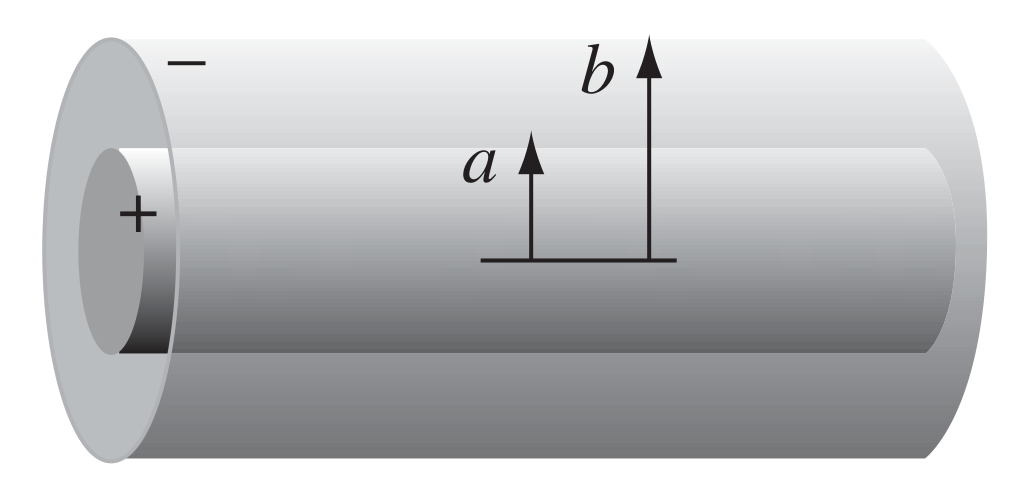
\includegraphics[width=0.5\textwidth]{imagenes/problema_24.png}
    \pagenumbering{gobble} % Desactiva la numeración de páginas
    \caption*{\label{fig:problema_24}Configuración del problema 2.16}
\end{figure}


Del Problema 2.16 tenemos que el potencial en el interior del cilindro de radio a es:
\[
\mathbf{E} = \frac{\rho s}{2\epsilon_o }  \hat{s}
\]

para \( a < s < b \) tenemos:
\[
\mathbf{E} = \frac{\rho a^2}{2\epsilon_o s }  \hat{s}
\]
% insertar figura del campo eléctrico

La diferencia de potencial entre un punto en el eje y un punto en el cilindro exterior es:
\[
\mathbf{V(a)}-\mathbf{V(b)}   = -\int_{a}^{b} \mathbf{E}\cdot d \mathbf{l}  
\]
Dado el intervalo de integración se puede separar la integral en dos partes:

Desde  \(a < s < b\) y  \(0 < s <a\)
\begin{align*}
    \mathbf{V(0)}-\mathbf{V(b)}   &= -\int_{a}^{b} \frac{\rho a^2}{2\epsilon_o s } ds - \int_{0}^{a} \frac{\rho s}{2\epsilon_o } ds \\
    &= -\left[\frac{\rho a^2}{2\epsilon_o} \ln(s) \right]_{a}^{b} - \left[\frac{\rho s^2}{4\epsilon_o} \right]_{0}^{a} \\
    &= -\frac{\rho a^2}{2\epsilon_o} \left[\ln(b) -\ln(a)  \right] - \left[\frac{\rho a^2}{4\epsilon_o} + 0 \right] \\
    &= -\left[\frac{\rho a^2}{2\epsilon_o} \ln{\frac{b}{a} } \right] - \left[\frac{\rho a^2}{4\epsilon_o} \right] \\
    &= -\frac{\rho a^2}{2\epsilon_o} \ln{\frac{b}{a} } - \frac{\rho a^2}{4\epsilon_o}\\
    &= -\frac{\rho a^2}{4\epsilon_o} \left(2\ln{\frac{b}{a} } + 1 \right) \\
\end{align*}


\end{document}
